\section{Architektur der Anwendung}\label{sec:architektur}

Die im letzten Kapitel vorgestellten theoretischen Konzepte sollen nun in die Praxis umgesetzt werden.
Dazu wird in diesem Kapitel die Architektur hinter der Anwendung erläutert sowie die Funktionsweise der Komponenten erklärt.

\subsection{Grundlegende Komponenten}

Die Anwendung kann in vier Hauptkomponenten eingeteilt werden: \textit{EGraph}, \textit{Service}, \textit{Server} und \textit{Weboberfläche}.
Abbildung~\ref{fig:architektur} zeigt den Zusammenhang zwischen diesen Komponenten. 

Die erste Komponente (\textit{E-Graph}) ist für die Erstellung und Verwaltung der E-Graph Datenstruktur zuständig. Dafür existieren sechs Klassen:
\textit{AbstractSyntaxTreeNode}, \textit{AbstractSyntaxTree}, \textit{RewriteRule}, \textit{ENode}, \textit{EClass} und \textit{EGraph}.
Die Klasse \textit{EGraph} enthält die Datenstruktur sowie einige weitere Funktionen, wie zum Beispiel die Visualisierung des E-Graph.
Sie ist abhängig von vier weiteren Klassen. Die beiden Klassen \textit{ENode} und \textit{EClass} repräsentieren E-Nodes und E-Classes.
Die Klasse \textit{RewriteRule} verkörpert eine rewrite rule, die aus einem linken und einem rechten Ausdruck besteht. Beide Ausdrücke werden in einen AST (\textbf{Abstract Syntax Tree}) umgewandelt, 
um das Anwenden der Regel auf den E-Graph zu vereinfachen.
Die letzte Abhängigkeit besteht von der Klasse \textit{AbstractSyntaxTree}. Sie stellt einen AST dar und benötigt dafür eine Klasse, 
die die Knoten repräsentiert (\textit{AbstractSyntaxTreeNode}).
Ein mathematischer Ausdruck, aus dem ein E-Graph entstehen soll, wird zuerst in einen AST umgewandelt. Dies vereinfacht später die Erstellung des E-Graphs.

Die zweite Komponente (\textit{Service}) ist für die Interaktion zwischen dem Server und der Datenstruktur verantwortlich. Die zuständige Klasse heißt \textit{EGraphService}. 
Von dieser wird eine Instanz beim Start des Servers erzeugt. 
Sie stellt dem Server Funktionen, wie zum Beispiel das Debugging, zur Verfügung und regelt die Sicherheitsüberprüfungen für Eingaben und Zustände. 

Die dritte Komponente (\textit{Server}) stellt das Backend der Anwendung dar. Sie enthält eine Datei \textit{server.py}, in der ein mit FastAPI erstellter Webserver
Anfragen der Weboberfläche entgegennimmt und zur Umsetzung der Anfragen mit dem Service interagiert. Da zwischen dem Server und der Weboberfläche Daten ausgetauscht werden
müssen, kommunizieren sie über das HTTP-Protokoll, während die Daten im JSON-Format übertragen werden.

Die vierte Komponente (\textit{Weboberfläche}) versieht die Anwendung mit einer Benutzeroberfläche, einer Dokumentation sowie der nötigen Kommunikation mit dem Server.
Die Benutzeroberfläche besteht aus einer Website (\textit{index.html}), die lokal im Browser läuft. Die Website erhält ihre Funktionalität durch die Funktionen in der 
Datei \textit{index.js}. Diese Datei schickt Anfragen an den Server und verarbeitet dessen Antworten, rendert den E-Graph und generiert Inhalte auf der Website. 
Die Dokumentation wurde separat mit \textit{Docusaurus} erstellt und erklärt die Installation der Anwendung, die Ausführung der Tests und die Bedienung der Benutzeroberfläche.  

\begin{figure}[H]
  \centering
  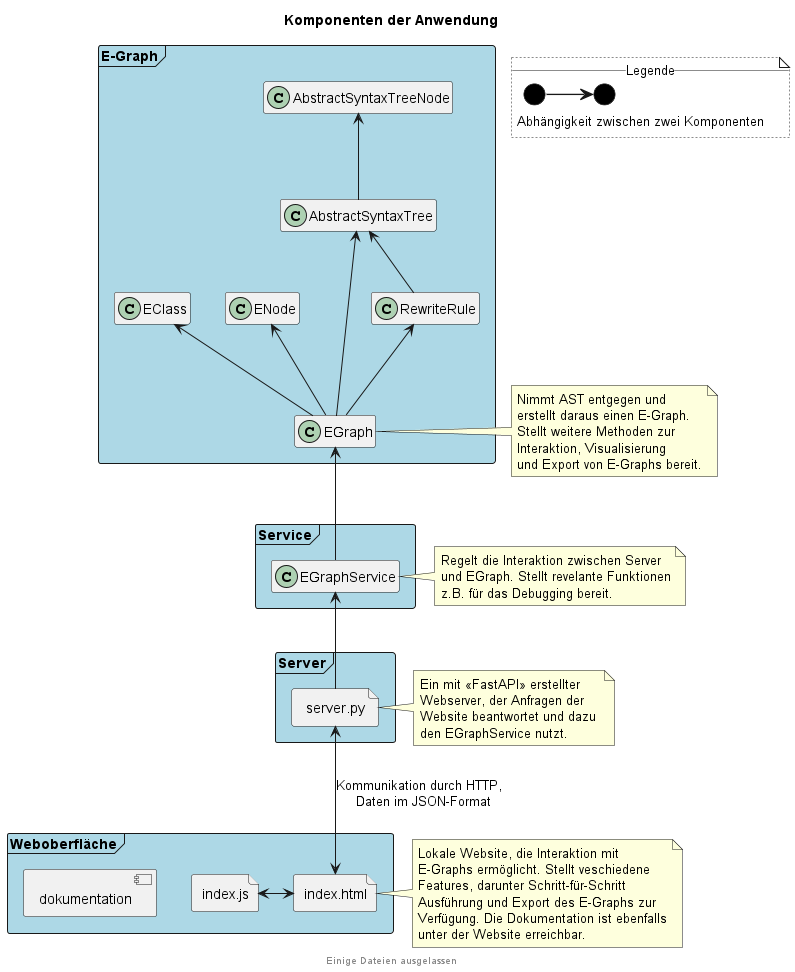
\includegraphics[scale=0.6]{../fig/components.png}
  \caption{Architekturdiagramm der Anwendung}
  \label{fig:architektur}
\end{figure}

\subsection{Kommunikation zwischen Server und Weboberfläche}

In diesem Abschnitt wird die Kommunikation zwischen Server, Weboberfläche und Benutzer stärker beleuchtet.
Hierzu zeigt Abbildung~\ref{fig:ablauf} die leicht vereinfachte Erstellung eines E-Graphs durch den Benutzer.

Die Interaktion startet mit der Eingabe eines Ausdrucks und dem Klicken auf den entsprechenden Button (Abb.~\ref{fig:ablauf}, Schritt 1) durch den Benutzer.
Das triggert die in JavaScript geschriebene Funktion \textit{create()}. 
Die Funktion \textit{create()} überprüft zuerst, ob der Service bereits einen E-Graph geladen hat (Abb.~\ref{fig:ablauf}, Schritt 2-3). Wenn dies der Fall ist, wird der Benutzer
gefragt, ob er diesen und alle mit ihm verbundenen Daten löschen möchte. Im Beispiel ist dieser Schritt nicht gezeigt.
Wenn der Benutzer dies bestätigt oder noch kein E-Graph im Service geladen ist, wird die Funktion \textit{createEGraph()} aufgerufen. 
Sie schickt per \textit{POST}-Request den Inhalt des Eingabefeldes an den Server (Abb.~\ref{fig:ablauf}, Schritt 4), der sich um die Erstellung kümmert.
Nach der Erstellung gibt die Antwort des Servers (Abb.~\ref{fig:ablauf}, Schritt 5) dem Benutzer Auskunft darüber (Abb.~\ref{fig:ablauf}, Schritt 6), ob das Erstellen des E-Graphs erfolgreich war.
Im nächsten Schritt muss die Benutzeroberfläche aktualisiert werden, um den E-Graph und die zugehörigen rewrite rules darzustellen.
Dafür ist die Funktion \textit{loadData()} verantwortlich, die auch bei einem erneuten Laden der Website dafür sorgt, dass die Inhalte weiterhin angezeigt werden.
In zwei Schritten lädt sie einmal den E-Graph und danach die rewrite rules.
Zunächst wird also eine \textit{GET}-Anfrage an den Server geschickt (Abb.~\ref{fig:ablauf}, Schritt 7), deren Antwort einen Status und die angeforderten Daten beinhaltet (Abb.~\ref{fig:ablauf}, Schritt 8).
In den Daten befindet sich der entsprechende E-Graph im \textit{DOT}-Format, der sogleich als SVG gerendert und auf 
der Weboberfläche angezeigt wird (Abb.~\ref{fig:ablauf}, Schritt 9).
Abschließend werden die Regeln durch eine weitere \textit{GET}-Anfrage geladen (Abb.~\ref{fig:ablauf}, Schritt 10-11). Zuletzt werden sie auf der Benutzeroberfläche gerendert (Abb.~\ref{fig:ablauf}, Schritt 12).

Insgesamt spiegelt die in Abbildung~\ref{fig:ablauf} dargestellte Vorgehensweise den Kommunikationsverlauf auch bei anderen Funktionen wider.
Dabei wurde beabsichtigt, die Kommunikation mit dem Server möglichst gering und effizient zu halten. Folglich konnte auf ein JavaScript-Framework verzichtet werden (siehe Kapitel~\ref{sec:entscheidungen}).

\begin{figure}[H]
  \centering
  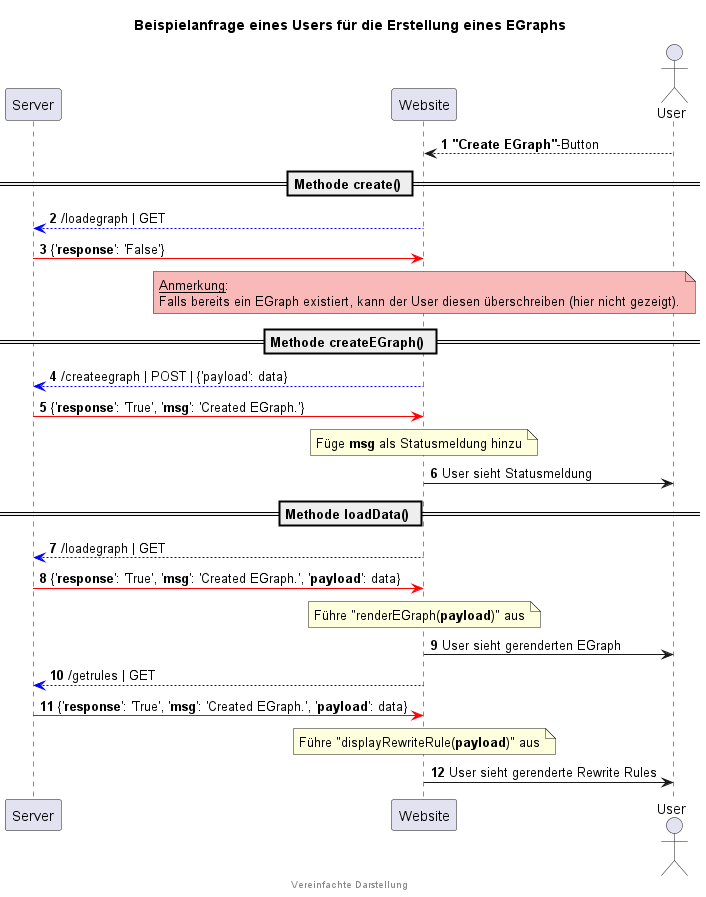
\includegraphics[scale=0.6]{../fig/query.png}
  \caption{Ablaufdiagramm der Kommunikation für die Erstellung eines E-Graphs zwischen Server, Weboberfläche und Benutzer}
  \label{fig:ablauf}
\end{figure}
